\documentclass[mathserif]{beamer}

\setbeamertemplate{frametitle}[default][center]%Centers the frame title.
\setbeamertemplate{navigation symbols}{}%Removes navigation symbols.
\setbeamertemplate{footline}{\raisebox{5pt}{\makebox[\paperwidth]{\hfill\makebox[10pt]{\scriptsize\insertframenumber}}}}
\setbeamertemplate{caption}[numbered]

\usepackage{amssymb,amsfonts,amsmath,latexsym,amsthm}
%\usepackage[usenames,dvipsnames]{color}
%\usepackage[]{graphicx}
%\usepackage[space]{grffile}
\usepackage{mathrsfs}   % fancy math font
% \usepackage[font=small,skip=0pt]{caption}
\usepackage[skip=0pt]{caption}
\usepackage{subcaption}
\usepackage{verbatim}
\usepackage{url}
\usepackage{bm}
\usepackage{dsfont}
\usepackage{extarrows}
\usepackage{multirow}
%\newcommand{\tth}   {\mbox{$\theta$}}
\newcommand{\thh}   {\mbox{$\theta$}}
\newcommand{\su}   {\mbox{$\sigma^2$}}
\newcommand{\so}   {\mbox{$\sigma_0^2$}}
\newcommand{\ko}   {\mbox{$\kappa_0$}}
\newcommand{\no}   {\mbox{$\nu_0$}}
\newcommand{\mo}   {\mbox{$\mu_0$}}
\newcommand{\ti}   {\mbox{$\tilde{x}$}}
\newcommand{\la}   {\mbox{$\lambda$}}
\newcommand{\bx}   {\mbox{$\bm{x}$}}
\newcommand{\bZ}   {\mbox{$\bm{Z}$}}
\newcommand{\bX}   {\mbox{$\bm{X}$}}
\newcommand{\bY}   {\mbox{$\bm{Y}$}}
\newcommand{\bA}   {\mbox{$\bm{A}$}}
\newcommand{\ba}   {\mbox{$\bm{a}$}}
\newcommand{\bb}   {\mbox{$\bm{b}$}}
\newcommand{\bt}   {\mbox{$\bm{t}$}}
\newcommand{\bz}   {\mbox{$\bm{z}$}}
\newcommand{\bw}   {\mbox{$\bm{w}$}}
\newcommand{\bbeta}   {\mbox{$\bm{\beta}$}}

\newcommand{\be}   {\mbox{$\bm{e}$}}
\newcommand{\bu}   {\mbox{$\bm{u}$}}
\newcommand{\bv}   {\mbox{$\bm{v}$}}
\newcommand{\sig}   {\mbox{$\Sigma$}}
\newcommand{\sigx}   {\mbox{$\Sigma_{XX}$}}
\newcommand{\sigxy}   {\mbox{$\Sigma_{XY}$}}
\newcommand{\tr}   {\mbox{$\text{tr}$}}
\newcommand{\ddet}   {\mbox{$\text{det}$}}
\newcommand\independent{\protect\mathpalette{\protect\independenT}{\perp}}
\def\independenT#1#2{\mathrel{\rlap{$#1#2$}\mkern2mu{#1#2}}}

\newcommand{\Expect}[1]{\ensuremath{\mathbf{E}\left[ #1 \right]}}
%\newcommand{\Var}[1]{\ensuremath{\mathrm{Var}\left[ #1 \right]}}
%\newcommand{\Cov}[1]{\ensuremath{\mathrm{Cov}\left[ #1 \right]}}
\newcommand{\MSE}{\ensuremath{\mathrm{MSE}}}
\newcommand{\RSS}{\ensuremath{\mathrm{RSS}}}
\newcommand{\Prob}[1]{\ensuremath{\mathrm{Pr}\left( #1 \right)}}
\newcommand{\ProbEst}[1]{\ensuremath{\widehat{\mathrm{Pr}}\left( #1 \right)}}
\DeclareMathOperator*{\argmin}{argmin} % thanks, wikipedia!
\DeclareMathOperator*{\argmax}{argmax} % thanks, wikipedia!
\DeclareMathOperator*{\sgn}{sgn} % thanks, wikipedia!

\newcommand{\lam}{\lambda}
\newcommand{\bmu}{\bm{\mu}}
%\newcommand{\bx}{\ensuremath{\mathbf{X}}}
\newcommand{\X}{\ensuremath{\mathbf{X}}}
\newcommand{\w}{\ensuremath{\mathbf{w}}}
\newcommand{\h}{\ensuremath{\mathbf{h}}}
\newcommand{\V}{\ensuremath{\mathbf{V}}}
%\newcommand{\tr}{\operatorname{tr}}

%\newcommand{\bx}{\ensuremath{\mathbf{X}}}
%\newcommand{\X}{\ensuremath{\mathbf{x}}}
%\newcommand{\w}{\ensuremath{\mathbf{w}}}
%\newcommand{\h}{\ensuremath{\mathbf{h}}}
%\newcommand{\V}{\ensuremath{\mathbf{v}}}
%\newcommand{\Cov}{\text{Cov}}
%\newcommand{\Var}{\text{Var}}

\DeclareMathOperator{\var}{Var}
\DeclareMathOperator{\cov}{Cov}
\newcommand{\Var}[1]{\ensuremath{\mathrm{Var}\left[ #1 \right]}}
\newcommand{\Cov}[1]{\ensuremath{\mathrm{Cov}\left[ #1 \right]}}


\newcommand{\indep}{\rotatebox{90}{\ensuremath{\models}}}
\newcommand{\notindep}{\not\hspace{-.05in}\indep}







\usepackage{float,bm}
\floatstyle{boxed}
\newfloat{code}{tp}{code}
\floatname{code}{Code Example}
%\newcommand{\tth}   {\mbox{$\theta$}}
\newcommand{\thh}   {\mbox{$\theta$}}
\newcommand{\su}   {\mbox{$\sigma^2$}}
\newcommand{\so}   {\mbox{$\sigma_0^2$}}
\newcommand{\ko}   {\mbox{$\kappa_0$}}
\newcommand{\no}   {\mbox{$\nu_0$}}
\newcommand{\mo}   {\mbox{$\mu_0$}}
\newcommand{\ti}   {\mbox{$\tilde{x}$}}
\newcommand{\la}   {\mbox{$\lambda$}}
\newcommand{\bx}   {\mbox{$\bm{x}$}}
\newcommand{\bZ}   {\mbox{$\bm{Z}$}}
\newcommand{\bX}   {\mbox{$\bm{X}$}}
\newcommand{\bY}   {\mbox{$\bm{Y}$}}
\newcommand{\bA}   {\mbox{$\bm{A}$}}
\newcommand{\ba}   {\mbox{$\bm{a}$}}
\newcommand{\bb}   {\mbox{$\bm{b}$}}
\newcommand{\bt}   {\mbox{$\bm{t}$}}
\newcommand{\bz}   {\mbox{$\bm{z}$}}
\newcommand{\bw}   {\mbox{$\bm{w}$}}
\newcommand{\bbeta}   {\mbox{$\bm{\beta}$}}

\newcommand{\be}   {\mbox{$\bm{e}$}}
\newcommand{\bu}   {\mbox{$\bm{u}$}}
\newcommand{\bv}   {\mbox{$\bm{v}$}}
\newcommand{\sig}   {\mbox{$\Sigma$}}
\newcommand{\sigx}   {\mbox{$\Sigma_{XX}$}}
\newcommand{\sigxy}   {\mbox{$\Sigma_{XY}$}}
\newcommand{\tr}   {\mbox{$\text{tr}$}}
\newcommand{\ddet}   {\mbox{$\text{det}$}}
\newcommand\independent{\protect\mathpalette{\protect\independenT}{\perp}}
\def\independenT#1#2{\mathrel{\rlap{$#1#2$}\mkern2mu{#1#2}}}

\newcommand{\Expect}[1]{\ensuremath{\mathbf{E}\left[ #1 \right]}}
%\newcommand{\Var}[1]{\ensuremath{\mathrm{Var}\left[ #1 \right]}}
%\newcommand{\Cov}[1]{\ensuremath{\mathrm{Cov}\left[ #1 \right]}}
\newcommand{\MSE}{\ensuremath{\mathrm{MSE}}}
\newcommand{\RSS}{\ensuremath{\mathrm{RSS}}}
\newcommand{\Prob}[1]{\ensuremath{\mathrm{Pr}\left( #1 \right)}}
\newcommand{\ProbEst}[1]{\ensuremath{\widehat{\mathrm{Pr}}\left( #1 \right)}}
\DeclareMathOperator*{\argmin}{argmin} % thanks, wikipedia!
\DeclareMathOperator*{\argmax}{argmax} % thanks, wikipedia!
\DeclareMathOperator*{\sgn}{sgn} % thanks, wikipedia!

\newcommand{\lam}{\lambda}
\newcommand{\bmu}{\bm{\mu}}
%\newcommand{\bx}{\ensuremath{\mathbf{X}}}
\newcommand{\X}{\ensuremath{\mathbf{X}}}
\newcommand{\w}{\ensuremath{\mathbf{w}}}
\newcommand{\h}{\ensuremath{\mathbf{h}}}
\newcommand{\V}{\ensuremath{\mathbf{V}}}
%\newcommand{\tr}{\operatorname{tr}}

%\newcommand{\bx}{\ensuremath{\mathbf{X}}}
%\newcommand{\X}{\ensuremath{\mathbf{x}}}
%\newcommand{\w}{\ensuremath{\mathbf{w}}}
%\newcommand{\h}{\ensuremath{\mathbf{h}}}
%\newcommand{\V}{\ensuremath{\mathbf{v}}}
%\newcommand{\Cov}{\text{Cov}}
%\newcommand{\Var}{\text{Var}}

\DeclareMathOperator{\var}{Var}
\DeclareMathOperator{\cov}{Cov}
\newcommand{\Var}[1]{\ensuremath{\mathrm{Var}\left[ #1 \right]}}
\newcommand{\Cov}[1]{\ensuremath{\mathrm{Cov}\left[ #1 \right]}}


\newcommand{\indep}{\rotatebox{90}{\ensuremath{\models}}}
\newcommand{\notindep}{\not\hspace{-.05in}\indep}






%\usepackage{fontspec}
%\setmainfont{Tahoma}

%\newcommand{\lam}{\lambda}
%\newcommand{\bmu}{\bm{\mu}}
%%\newcommand{\bx}{\ensuremath{\mathbf{X}}}
%\newcommand{\X}{\ensuremath{\mathbf{x}}}
%\newcommand{\w}{\ensuremath{\mathbf{w}}}
%\newcommand{\h}{\ensuremath{\mathbf{h}}}
%\newcommand{\V}{\ensuremath{\mathbf{v}}}
%\newcommand{\cov}{\text{Cov}}
%\newcommand{\var{\text{Var}}}

%\DeclareMathOperator{\var}{Var}
%\DeclareMathOperator{\cov}{Cov}

%\newcommand{\indep}{\rotatebox{90}{\ensuremath{\models}}}
%\newcommand{\notindep}{\not\hspace{-.05in}\indep}

\usepackage{graphicx} %The mode "LaTeX => PDF" allows the following formats: .jpg  .png  .pdf  .mps
\graphicspath{{./PresentationPictures/}} %Where the figures folder is located
\usepackage{listings}
\usepackage{media9}
\usepackage{movie15}
\addmediapath{./Movies/}

\newcommand{\beginbackup}{
   \newcounter{framenumbervorappendix}
   \setcounter{framenumbervorappendix}{\value{framenumber}}
}
\newcommand{\backupend}{
   \addtocounter{framenumbervorappendix}{-\value{framenumber}}
   \addtocounter{framenumber}{\value{framenumbervorappendix}} 
}


%\usepackage{algorithm2e}
\usepackage[ruled,lined]{algorithm2e}
\def\algorithmautorefname{Algorithm}
\SetKwIF{If}{ElseIf}{Else}{if}{then}{else if}{else}{endif}
%\usepackage{times}
%\usepackage[tbtags]{amsmath}
%\usepackage{amssymb}
\usepackage{amsfonts}
%\usepackage{slfortheorems}
\usepackage{epsfig}
\usepackage{graphicx}
%\usepackage[small]{caption}
%\usepackage[square]{natbib}
%\newcommand{\newblock}{}
%\bibpunct{(}{)}{;}{a}{}{,}
%\bibliographystyle{ims}
%\usepackage[letterpaper]{geometry}
%\usepackage{color}
%\setlength{\parindent}{0pt}

\usepackage{natbib}
\bibpunct{(}{)}{;}{a}{}{,}
%\usepackage{hyperref}

\DeclareMathOperator*{\Exp}{Exp}
\DeclareMathOperator*{\TExp}{TExp}
\DeclareMathOperator*{\Bernoulli}{Bernoulli}
\DeclareMathOperator*{\Beta}{Beta}
\DeclareMathOperator*{\Ga}{Gamma}
\DeclareMathOperator*{\TGamma}{TGamma}
\DeclareMathOperator*{\Poisson}{Poisson}
\DeclareMathOperator*{\Binomial}{Binomial}
\DeclareMathOperator*{\NormalGamma}{NormalGamma}
\DeclareMathOperator*{\InvGamma}{InvGamma}
\DeclareMathOperator*{\Cauchy}{Cauchy}
\DeclareMathOperator*{\Uniform}{Uniform}
\DeclareMathOperator*{\Gumbel}{Gumbel}
\DeclareMathOperator*{\Pareto}{Pareto}
\DeclareMathOperator*{\Mono}{Mono}
\DeclareMathOperator*{\Geometric}{Geometric}
\DeclareMathOperator*{\Wishart}{Wishart}

\newcommand{\N}{\mathcal{N}}

\newcommand{\R}{\mathbb{R}}
\newcommand{\Z}{\mathbb{Z}}
\newcommand{\E}{\mathbb{E}}
\renewcommand{\Pr}{\mathbb{P}}
\newcommand{\I}{\mathds{1}}
\newcommand{\V}{\mathbb{V}}

% Math operators
\DeclareMathOperator*{\diag}{diag}
\DeclareMathOperator*{\median}{median}
\DeclareMathOperator*{\Vol}{Vol}

% Miscellaneous commands
\newcommand{\iid}{\stackrel{\mathrm{iid}}{\sim}}
\newcommand{\matrixsmall}[1]{\bigl(\begin{smallmatrix}#1\end{smallmatrix} \bigr)}

\newcommand{\items}[1]{\begin{itemize} #1 \end{itemize}}

\newcommand{\todo}[1]{\emph{\textcolor{red}{(#1)}}}

\newcommand{\branch}[4]{
\left\{
	\begin{array}{ll}
		#1  & \mbox{if } #2 \\
		#3 & \mbox{if } #4
	\end{array}
\right.
}

% approximately proportional to
\def\app#1#2{%
  \mathrel{%
    \setbox0=\hbox{$#1\sim$}%
    \setbox2=\hbox{%
      \rlap{\hbox{$#1\propto$}}%
      \lower1.3\ht0\box0%
    }%
    \raise0.25\ht2\box2%
  }%
}
\def\approxprop{\mathpalette\app\relax}

\newcommand{\btheta}{{\bm\theta}}
\newcommand{\bbtheta}{{\pmb{\bm\theta}}}

%\usepackage{zref-savepos}
%
%\newcounter{restofframe}
%\newsavebox{\restofframebox}
%\newlength{\mylowermargin}
%\setlength{\mylowermargin}{2pt}
%
%\newenvironment{restofframe}{%
%    \par%\centering
%    \stepcounter{restofframe}%
%    \zsavepos{restofframe-\arabic{restofframe}-begin}%
%    \begin{lrbox}{\restofframebox}%
%}{%
%    \end{lrbox}%
%    \setkeys{Gin}{keepaspectratio}%
%    \raisebox{\dimexpr-\height+\ht\strutbox\relax}[0pt][0pt]{%
%    \resizebox*{!}{\dimexpr\zposy{restofframe-\arabic{restofframe}-begin}sp-\zposy{restofframe-\arabic{restofframe}-end}sp-\mylowermargin\relax}%
%        {\usebox{\restofframebox}}%
%    }%
%    \vskip0pt plus 1filll\relax
%    \mbox{\zsavepos{restofframe-\arabic{restofframe}-end}}%
%    \par
%}


\usepackage{tikz}
\usetikzlibrary{arrows}

%\usepackage[usenames,dvipsnames]{xcolor}
\usepackage{tkz-berge}
\usetikzlibrary{fit,shapes}

\usepackage{calc}
%%
%% The tikz package is used for doing the actual drawing.
%\usepackage{tikz}
%%
%% In order to be able to put arrowheads in the middle of directed edges, we need an extra library.
\usetikzlibrary{decorations.markings}
%%
%% The next line says how the "vertex" style of nodes should look: drawn as small circles.
\tikzstyle{vertex}=[circle, draw, inner sep=0pt, minimum size=6pt]
%%
%% Next, we make a \vertex command as a shorthand in place of \node[vertex} to get that style.
\newcommand{\vertex}{\node[vertex]}
%%
%% Finally, we declare a "counter", which is what LaTeX calls an integer variable, for use in
%% the calculations of angles for evenly spacing vertices in circular arrangements.
\newcounter{Angle}

\newtheoremstyle{example}
{\topsep} % space above
{\topsep} % space below
{} % body font
{} % indent
{\bf} % head font
{:} % punctuation between head and body
{0.5em} % space after head
{} % manually specify head
%{\thmname{#1}\thmnumber{ #2}\thmnote{:#3}} % manually specify head

\theoremstyle{example}
\newtheorem{ex}{Example}[section]

\newtheoremstyle{definition}
{\topsep} % space above
{\topsep} % space below
{} % body font
{} % indent
{\sc} % head font
{:} % punctuation between head and body
{0.5em} % space after head
{} % manually specify head
%{\thmname{#1}\thmnumber{ #2}\thmnote{:#3}} % manually specify head

\theoremstyle{definition}
\newtheorem{defn}{Definition}[section]

\theoremstyle{rem}
\newtheorem{rem}{Remark}[section]

\newtheoremstyle{theorem}
{\topsep} % space above
{\topsep} % space below
{} % body font
{} % indent
{\sc} % head font
{:} % punctuation between head and body
{0.5em} % space after head
{} % manually specify head
%{\thmname{#1}\thmnumber{ #2}\thmnote{:#3}} % manually specify head

\theoremstyle{theorm}
\newtheorem{thm}{Theorem}[section]



%%%to add in new counter for slides in beamer

%\setbeamertemplate{footline}{
%  \leavevmode%
%  \hbox{%
%  \begin{beamercolorbox}[wd=.333333\paperwidth,ht=2.25ex,dp=1ex,center]{author in head/foot}%
%    \usebeamerfont{author in head/foot}\insertshortauthor~~(\insertshortinstitute)
%  \end{beamercolorbox}%
%  \begin{beamercolorbox}[wd=.333333\paperwidth,ht=2.25ex,dp=1ex,center]{title in head/foot}%
%    \usebeamerfont{title in head/foot}\insertshorttitle
%  \end{beamercolorbox}%
%  \begin{beamercolorbox}[wd=.333333\paperwidth,ht=2.25ex,dp=1ex,right]{date in head/foot}%
%    \usebeamerfont{date in head/foot}\insertshortdate{}\hspace*{2em}
%    \insertframenumber{} \hspace*{2ex} % hier hat's sich ge�ndert
%  \end{beamercolorbox}}%
%  \vskip0pt%
%}



%%%%%

\newcommand*\oldmacro{}
\let\oldmacro\insertshortauthor
\renewcommand*\insertshortauthor{
  \leftskip=.3cm
\insertframenumber\,/\,\inserttotalframenumber\hfill\oldmacro}




%\excludecomment{notbeamer}
%\includecomment{beamer}



\title{The Multi Stage Gibbs Sampling: Data Augmentation Dutch Example}
\author{Rebecca C. Steorts \\ Bayesian Methods and Modern Statistics: STA 360/601}
\date{Module 8}

\begin{document}

\maketitle

\frame{
\frametitle{Example: Data augmentation / Auxiliary variables}
\begin{itemize}
\item A commonly-used technique for designing MCMC samplers is to use \emph{data augmentation}, also known as \emph{auxiliary variables}.
\item Introduce variable(s) $Z$ that depends on the distribution of the existing variables in such a way that the
resulting conditional distributions, with $Z$ included, are easier to sample from and/or result in better mixing.
\item  $Z$'s are latent/hidden variables that are introduced for the purpose of simplifying/improving the sampler.
\end{itemize}
}

\frame{
Idea: Create Z's and throw them away at the end! 
\begin{itemize}
\item Suppose we want to sample from $p(x,y)$, but $p(x|y)$ and/or $p(y|x)$ are complicated. 
\item Choose $$p(z|x,y)$$ such
that $p(x|y,z)$, $p(y|x,z)$, and $p(z|x,y)$ are easy to sample from. 
\item Then construct a Gibbs sampler to sample all three variables
$(X,Y,Z)$ from $p(x,y,z)$.
\item Then we just throw away the $Z$'s and we will have samples $(X,Y)$ from $p(x,y)$.
\end{itemize}

}

\frame{
\frametitle{Dutch Example}


Consider a data set on the heights of 695 Dutch women and 562 Dutch men.  

\vskip 1em

Suppose we have the list of heights, but we don't know which data points
are from women and which are from men.  

}

\frame{

From Figure \ref{figure:heights-combined} can we still infer the distribution of female heights and male heights?

\begin{figure}
  \begin{center}
    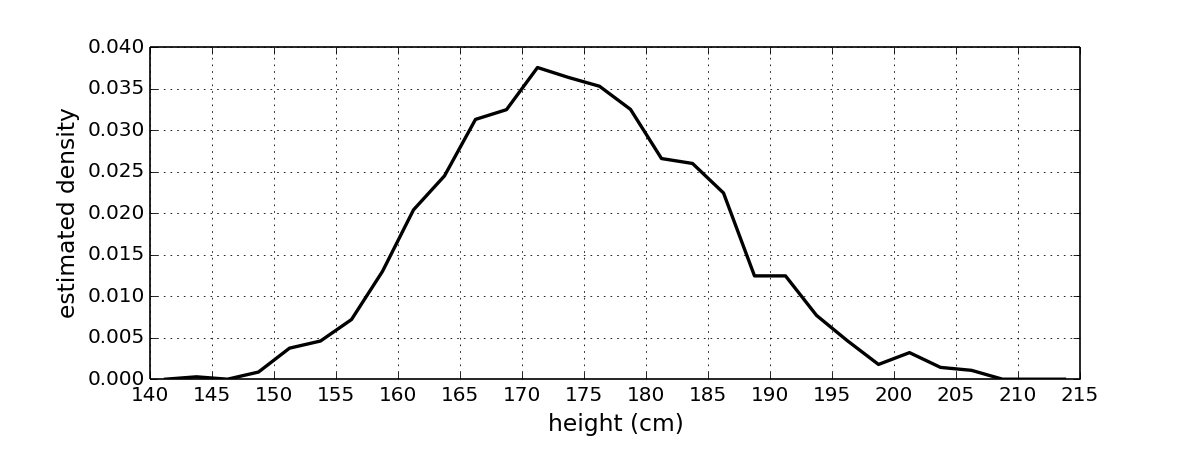
\includegraphics[width=1\textwidth]{examples/heights-combined}
    % Source: Original work by J. W. Miller.
  \end{center}
  \caption{Heights of Dutch women and men, combined.}
  \label{figure:heights-combined}
\end{figure}

\pause
% todo: we don't exactly do this...
Surprisingly, the answer is yes!

}

\frame{
What's the magic trick?
\vskip 1em

The reason is that this is a two-component mixture of Normals,
and there is an (essentially) unique set of mixture parameters corresponding to any such distribution.

\vskip 1em

We'll get to details soon. Be patient!



}

\frame{
\frametitle{Constructing a Gibbs sampler}
To construct a Gibbs sampler for this situation:

\begin{itemize}
\item Common to introduce an auxiliary variable $Z_i$ for each datapoint,
indicating which mixture component it is drawn from.
\item  In this example, $Z_i$ indicates whether subject $i$ is female or male.
\item This results in a Gibbs sampler that is easy to derive/implement.
\end{itemize}



}

\frame{
\frametitle{Two component Mixture Model}


Let's assume that both mixture components (female and male) have the same precision, say $\lambda$, and that $\lambda$ is fixed and known.  

\vskip 1em

Then the usual two-component Normal mixture model is:
\begin{align}
  & X_1,\ldots,X_n|\mu,\pi\,\iid\,F(\mu,\pi)\\
    & \mu:=(\mu_0,\mu_1) \iid \N(m,\ell^{-1})\\
    & \pi \sim \Beta(a,b)
\end{align}
where $F(\mu,\pi)$ is the distribution with p.d.f. 
$$ f(x|\mu,\pi) = (1-\pi)\N(x\mid \mu_0,\lambda^{-1}) + \pi\N(x\mid \mu_1,\lambda^{-1}) $$
and $\mu=(\mu_0,\mu_1)$.
}

\frame{
The likelihood is
\begin{align*}
    p(x_{1:n}|\mu,\pi) &= \prod_{i=1}^n f(x_i|\mu,\pi) \\
                       & = \prod_{i=1}^n \Big[ (1-\pi)\N(x_i\mid \mu_0,\lambda^{-1}) + \pi\N(x_i\mid \mu_1,\lambda^{-1}) \Big] 
\end{align*}
which is a complicated function of $\mu$ and $\pi$, making the posterior difficult to sample from directly.


}

\frame{
\frametitle{Latent allocation variables to the rescue!}

Define an equivalent model that includes latent ``allocation'' variables $Z_1,\ldots,Z_n$
\vskip 1em

These indicate which mixture component each data point
comes from--that is, $Z_i$ indicates whether subject $i$ is female or male.
\begin{align}
 & X_i\sim\N(\mu_{Z_i},\lambda^{-1}) \text{ independently for } i=1,\ldots,n.\\
     & Z_1,\ldots,Z_n|\mu,\pi\,\iid\,\Bernoulli(\pi)\\
    & \mu= (\mu_0,\mu_1) \iid \N(m,\ell^{-1})\\
    & \pi \sim \Beta(a,b)
\end{align}
}

\frame{
Recall
\textcolor{blue}{
\begin{align*}
 & X_i\sim\N(\mu_{Z_i},\lambda^{-1}) \text{ independently for } i=1,\ldots,n.\\
     & Z_1,\ldots,Z_n|\mu,\pi\,\iid\,\Bernoulli(\pi)\\
    & \mu= (\mu_0,\mu_1) \iid \N(m,\ell^{-1})\\
    & \pi \sim \Beta(a,b)
\end{align*}
}
This is equivalent to the model above, since
\begin{align}
    &p(x_i|\mu,\pi) \\
    &= p(x|Z_i=0,\mu,\pi)\Pr(Z_i=0|\mu,\pi) 
                    + p(x|Z_i=1,\mu,\pi)\Pr(Z_i=1|\mu,\pi) \\
            &= (1-\pi)\N(x_i|\mu_0,\lambda^{-1}) + \pi\N(x_i|\mu_1,\lambda^{-1})\\
            &= f(x_i|\mu,\pi),
\end{align}
and thus it induces the same distribution on $(x_{1:n},\mu,\pi)$. The latent model is considerably easier to work with, particularly for Gibbs
sampling. 



}

\frame{
\frametitle{Full conditionals}
Derive the full conditionals below as an exercise. 
\vskip 1em
Denote $x=x_{1:n}$ and $z=z_{1:n}$. 
\begin{itemize}
\item Find ($\pi|\cdots$) 
\item Find ($\mu|\cdots$) 
\item Find ($z|\cdots$)
\end{itemize}
As usual, each iteration of Gibbs sampling proceeds by sampling from each of these conditional distributions, in turn.
\vskip 1em
They are in this module, so you can check your results after completion. 


}

\frame{
\frametitle{Full conditionals derived}
\begin{itemize}
    \item ($\pi|\cdots$) Given $z$, $\pi$ is independent of everything else, so this reduces to a Beta--Bernoulli model, and we have
        $$ p(\pi|\mu,z,x) = p(\pi|z) =\Beta(\pi\mid a + n_1,\, b + n_0) $$
        where $n_k = \sum_{i=1}^n \I(z_i=k)$ for $k \in \{0, 1\}$.
        \end{itemize}
        }
        
\frame{
\begin{itemize}        
    \item ($\mu|\cdots$) Given $z$, we know which component each data point comes from. 
    \vskip 1em
    The model (conditionally on $z$) is just two
        independent Normal--Normal models, as we have seen before:
        \begin{align*}
            \bm\mu_0|\mu_1,x,z,\pi\, \sim \,\N(M_0,L_0^{-1})\\
            \bm\mu_1|\mu_0,x,z,\pi\, \sim \,\N(M_1,L_1^{-1})
        \end{align*}
        where for $k\in\{0,1\}$,
        \begin{align*}
        n_k &= \sum_{i=1}^n \I(z_i=k)\\
        L_k &=\ell + n_k\lambda\\
        M_k &=\frac{\ell m + \lambda\sum_{i:z_i=k} x_i}{\ell + n_k\lambda}.
        \end{align*}
        \end{itemize}
        }
        
        \frame{
\begin{itemize}
    \item ($z|\cdots$)
        \begin{align*}
            p(z|\mu,\pi,x)&\underset{z}{\propto}p(x,z,\pi,\mu)\underset{z}{\propto} p(x|z,\mu) p(z|\pi)\\
            & =\prod_{i = 1}^n \N(x_i|\mu_{z_i},\lambda^{-1})\Bernoulli(z_i|\pi)\\
            & =\prod_{i = 1}^n \Big(\pi\N(x_i|\mu_1,\lambda^{-1})\Big)^{z_i} \Big((1-\pi)\N(x_i|\mu_0,\lambda^{-1})\Big)^{1-z_i}\\
            & =\prod_{i = 1}^n \alpha_{i,1}^{z_i} \alpha_{i,0}^{1-z_i}\\
            &\underset{z}{\propto}\prod_{i = 1}^n\Bernoulli(z_i\mid \alpha_{i,1}/(\alpha_{i,0}+\alpha_{i,1}))
        \end{align*}
        where
        \begin{align*}
            \alpha_{i,0} & =(1-\pi)\N(x_i|\mu_0,\lambda^{-1})\\
            \alpha_{i,1} & =\pi\N(x_i|\mu_1,\lambda^{-1}).
        \end{align*}
\end{itemize}
}

\frame{
\begin{figure}
    \centering
    \begin{subfigure}[t]{1\textwidth}
        \centering
        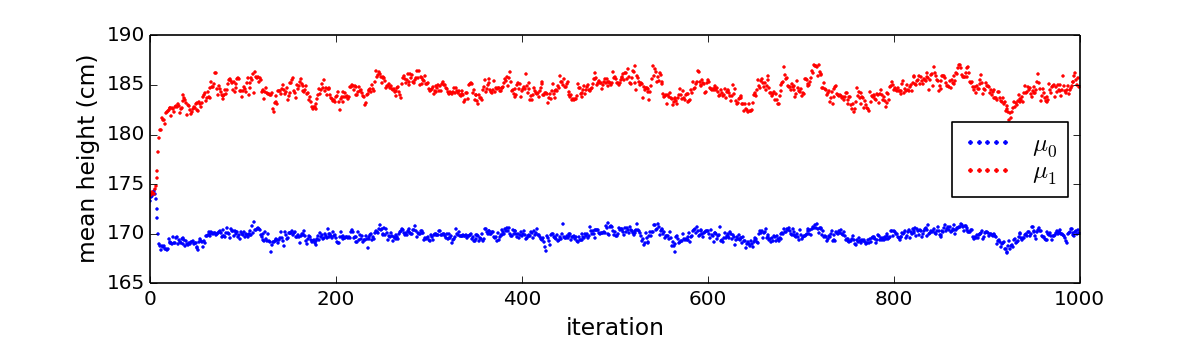
\includegraphics[trim=0 0.4cm 0 0, clip, width=\textwidth]{examples/mix-mu_trace-a.png}
        % Original work by Jeffrey W. Miller
        \caption{Traceplots of the component means, $\mu_0$ and $\mu_1$.}
    \end{subfigure}
    \begin{subfigure}[t]{1\textwidth}
        \centering
        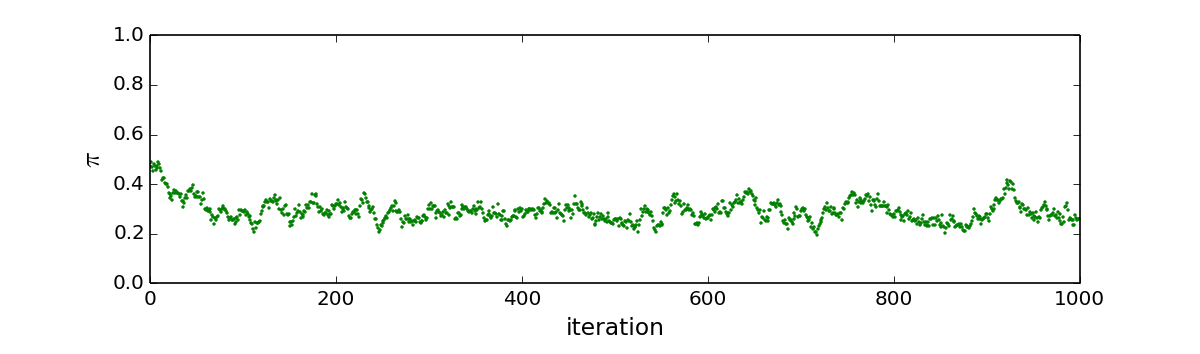
\includegraphics[trim=0 0.4cm 0 0, clip, width=\textwidth]{examples/mix-p_trace-a.png}
        % Original work by Jeffrey W. Miller
        \caption{Traceplot of the mixture weight, $\pi$ (prior probability that a subject comes from component 1).}
    \end{subfigure}
    \vspace{.5em}
    \caption{Results from one run of the mixture example.}
    \label{figure:mix}
\end{figure}
}

\frame{
\begin{figure}
    \centering
   \begin{subfigure}[t]{1\textwidth}
        \centering
        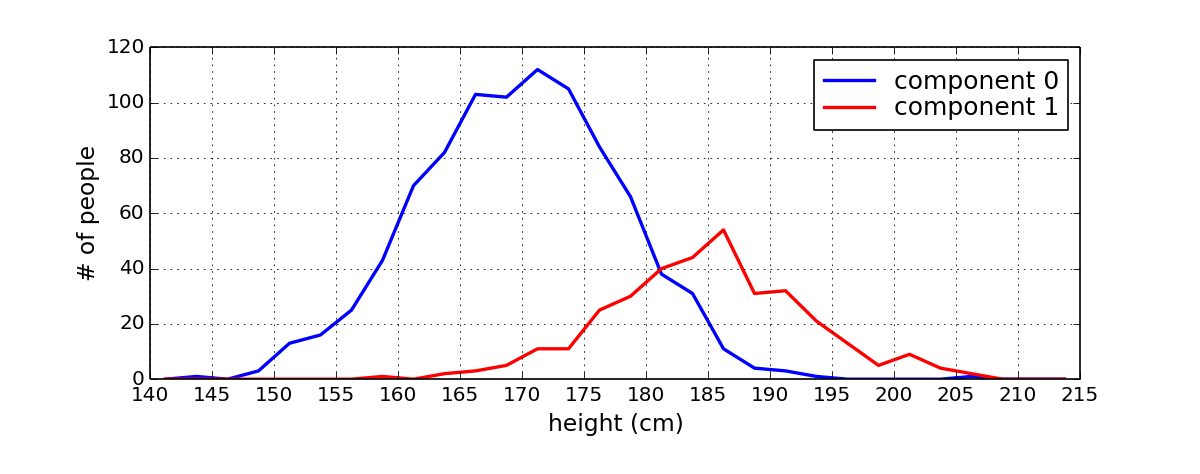
\includegraphics[trim=0 0.4cm 0 0, clip, width=\textwidth]{examples/mix-histograms_at_last_sample-a.png}
        % Original work by Jeffrey W. Miller
        \caption{Histograms of the heights of subjects assigned to each component, according to $z_1,\ldots,z_n$, in a typical sample.}
    \end{subfigure}
      \vspace{.5em}
    \caption{Results from one run of the mixture example. One way of visualizing the allocation/assignment variables $z_1,\ldots,z_n$ is to make histograms of the heights of the subjects assigned to each component. }
    \label{figure:mix}
\end{figure}
    }

\frame{
\frametitle{My Factory Settings!}
\begin{itemize}
\item $\lambda = 1/\sigma^2$ where $\sigma = 8$ cm ($\approx 3.1$ inches) ($\sigma$ = standard deviation of the subject heights within each component)
\item $a = 1$, $b = 1$ (Beta parameters, equivalent to prior ``sample size'' of 1 for each component)
\item $m = 175$ cm ($\approx 68.9$ inches) (mean of the prior on the component means)
\item $\ell = 1/s^2$ where $s = 15$ cm ($\approx 6$ inches) ($s$ = standard deviation of the prior on the component means)
\end{itemize}
}

\frame{
\frametitle{My Factory Settings!}
We initialize the sampler at:
\begin{itemize}
\item $\pi = 1/2$ (equal probability for each component)
\item $z_1,\ldots,z_n$ sampled i.i.d.\ from $\Bernoulli(1/2)$ (initial assignment to components chosen uniformly at random)
\item $\mu_0 =\mu_1 = m$ (component means initialized to the mean of their prior)
\end{itemize}
}

%\frame{
%Figure \ref{figure:mix} shows a few plots of the results for $N = 10^3$ iterations. (Note: This should probably be run for longer---this short run is simply for illustration purposes.) From the traceplots of $\mu_0$ and $\mu_1$, we see that one component quickly settles to have a mean of around 168--170 cm and the other to a mean of around 182--186 cm. Recalling that we are not using the true assignments of subjects to components (that is, we don't know whether they are male or female), it is interesting to note that this is fairly close to the sample averages: 168.0 cm (5 feet 6.1 inches) for females, and 181.4 cm (5 feet 11.4 inches) for males.
%
%The traceplot of $\pi$ indicates that the sampler is exploring values of around 0.2 to 0.4---that is, the proportion of people coming from group 1 is around 0.2 to 0.4. Meanwhile, looking at the actual labels (female and male), the empirical proportion of males is $562/(695+562) \approx 0.45$. So this is slightly off. This could be due to not having enough data, and/or due to the fact that we are assuming a fixed value of $\lambda$. It would be much better, and nearly as easy, to allow components 0 and 1 to have different precisions, $\lambda_0$ and $\lambda_1$, and put Gamma priors on them.
% 
%As shown in the bottom plot (panel (c)), one way of visualizing the allocation/assignment variables $z_1,\ldots,z_n$ is to make histograms of the heights of the subjects assigned to each component. At a glance, this shows us where the two clusters of datapoints are, how large each cluster is, and what shape they have.
%}

\frame{


\begin{figure}
    \centering
    \begin{subfigure}[t]{1\textwidth}
        \centering
        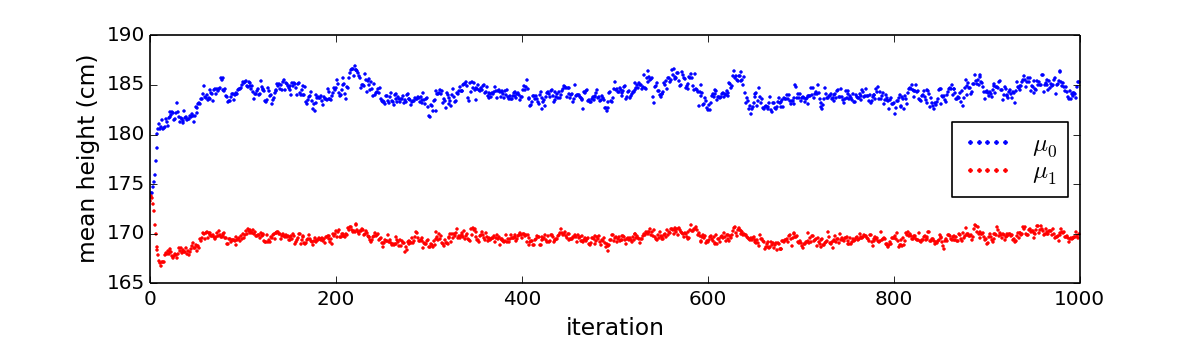
\includegraphics[trim=0 0.4cm 0 0, clip, width=1\textwidth]{examples/mix-mu_trace-b.png}
        % Original work by Jeffrey W. Miller
        \caption{Traceplots of the component means, $\mu_0$ and $\mu_1$.}
    \end{subfigure}
    \begin{subfigure}[t]{1\textwidth}
        \centering
        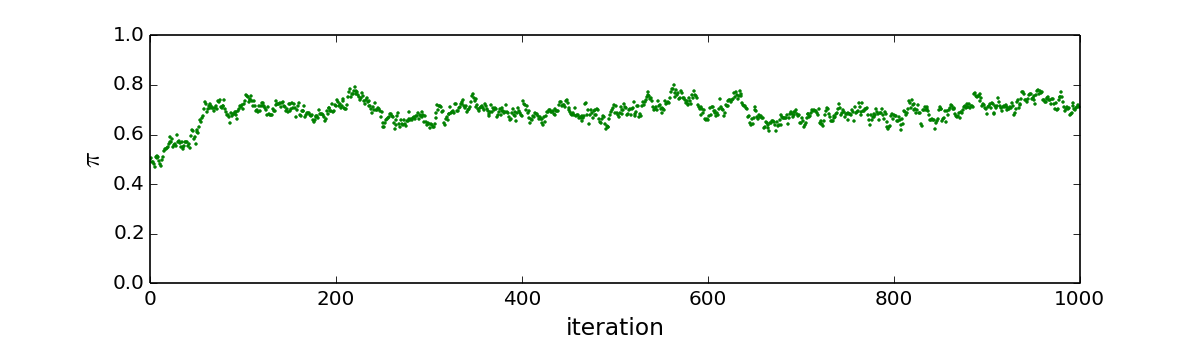
\includegraphics[trim=0 0.4cm 0 0, clip, width=1\textwidth]{examples/mix-p_trace-b.png}
        % Original work by Jeffrey W. Miller
        \caption{Traceplot of the mixture weight, $\pi$ (prior probability that a subject comes from component 1).}
    \end{subfigure}
       \caption{Results from another run of the mixture example.}
    \label{figure:mix-b}
\end{figure}
  }
  

  
  \frame{  
  \begin{figure}
   \centering
    \begin{subfigure}[t]{1\textwidth}
        \centering
        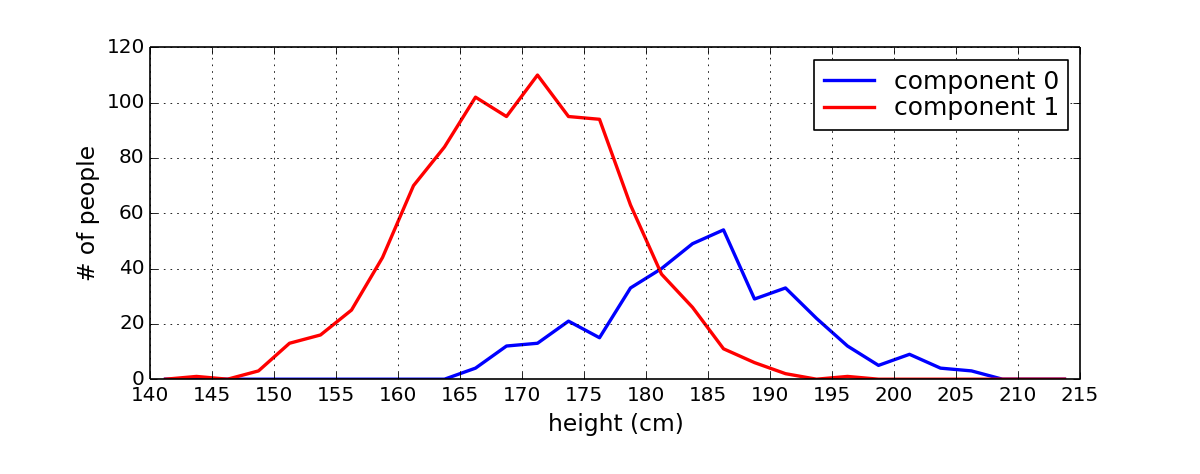
\includegraphics[trim=0 0.4cm 0 0, clip, width=1\textwidth]{examples/mix-histograms_at_last_sample-b.png}
        % Original work by Jeffrey W. Miller
        \caption{Histograms of the heights of subjects assigned to each component, according to $z_1,\ldots,z_n$, in a typical sample.}
    \end{subfigure}
    \vspace{.5em}
    \caption{Results from another run of the mixture example.}
    \label{figure:mix-b}
\end{figure}

}

\frame{
\frametitle{Caution -- watch out for modes}
Example illustrates a big thing that can go wrong with MCMC (although fortunately, in this case, the results are still valid if interpreted correctly). 
\begin{itemize}
\item Why are females assigned to component 0 and males assigned to component 1? Why not the other way around? 
\item In fact, the model is symmetric with respect to the two components, and thus the posterior is also symmetric. 
\item If we run the sampler multiple times (starting from the same initial values), sometimes it will settle on females as 0 and males as 1, and sometimes on females as 1 and males as 0 --- see Figure \ref{figure:mix-b}. 
\item Roughly speaking, the posterior has two modes.
\item  If the sampler were behaving properly, it would move back and forth between these two modes.
\item But it doesn't---it gets stuck in one and stays there.
\end{itemize}
}

\frame{


This is a very common problem with mixture models. Fortunately, however, in the case of mixture models, the results are still valid if we interpret them correctly. Specifically, our inferences will be valid as long as we only consider quantities that are invariant with respect to permutations of the components (e.g. symmetry about the mean).
}

















\end{document}